\documentclass[AutoFakeBold,AutoFakeSlant]{beamer}
\usepackage{ctex}
\usepackage{hyperref}
\usepackage[defaultsans]{droidsans}
\usepackage{fontspec}
\usepackage{newtxmath}
\usepackage{latexsym,amsmath,xcolor,multicol,booktabs,calligra,tcolorbox}
\usepackage{graphicx,tabularx,multirow,makecell}
\usepackage{listings}
\lstset{
    basicstyle=\ttfamily\tiny,
    breaklines=true,
    breakatwhitespace=true,
    columns=fullflexible,
    frame=single,
    backgroundcolor=\color{gray!6},
}
\usepackage{tikz}
\usetikzlibrary{arrows.meta,positioning}

\usetheme{Madrid}
\usecolortheme{default}
\setbeamertemplate{navigation symbols}{}
\setbeamertemplate{footline}[frame number]

%% 图资源：本地 figures、审计汇总图、流水线导出的各应用子目录（仅编译用，正文不展示路径）
\graphicspath{{./figures/}{./figures/audit/}{../src/output/run_20260413_150151/}}
\newcommand{\HandoutPdfRel}{../ref/system_design_expr_lab2_4_handout.pdf}

\author{李禹江，张博涵，蒋兴宇}
\title{隐私政策句级分析一体化流水线}
\subtitle{\texorpdfstring{聚类、少样本学习、人工送标与 Data Safety 句级审计}{实验方法汇报}}
\institute{我的刀盾队}
\date{2026-04-13}

\begin{document}
\kaishu

\begin{frame}
    \titlepage
    \vspace{0.5em}
\end{frame}

\begin{frame}
    \frametitle{目录}
    \tableofcontents
\end{frame}

%------------------------------------------------------------
\section{实验目的}

\begin{frame}
    \frametitle{实验目的}
    \begin{itemize}
        \item \textbf{句级结构化}：将多款应用隐私政策\textbf{切分为句子}，为每句赋予\textbf{文档与句序号}，便于检索、审计与可视化。
        \item \textbf{个信相关判别}：对每句做\textbf{二分类}（是否与\textbf{个人信息的处理与利用}实质相关），并用\textbf{规则弱信号}（关键词等）与模型结果对照。
        \item \textbf{Data Safety 风格句级审计}：在「披露侧—政策句」对比框架下输出 \textbf{incorrect / incomplete / inconsistent} 三标签，支撑合规差异分析。
        \item \textbf{主题维度分析}：句向量聚类 + 与个保法 22 项参考段的相似度，辅助\textbf{主题分布}与\textbf{政策—法条}对照。
        \item \textbf{人机协同}：对高优先级句子\textbf{送标}，由人在统一界面中写标签与备注；\textbf{人机分歧}可回收到\textbf{少样本示例库}，迭代改进分类边界。
    \end{itemize}
\end{frame}

%------------------------------------------------------------
\section{实验环境}

\begin{frame}
    \frametitle{实验环境}
    \begin{itemize}
        \item \textbf{系统}：Windows 10/11。
        \item \textbf{软件栈}：Python 3.10+；中文句向量嵌入（BGE 系）；降维（UMAP）、密度聚类（HDBSCAN）；可视化与批处理脚本。
        \item \textbf{嵌入与聚类}：采用 FlagEmbedding 管线加载 \textbf{BAAI/bge-small-zh-v1.5}，用于句向量、法参考段向量及后续降维聚类。
        \item \textbf{数据}：五款应用的隐私政策\textbf{中文原文}（UTF-8）：小红书、LOFTER、Blued 极速版、世纪佳缘、Soul。
    \end{itemize}
\end{frame}

%------------------------------------------------------------
\section{实验内容}

\begin{frame}
    \frametitle{实验流程总览（端到端）}
    \centering
    \begin{tikzpicture}[
        node distance=5mm and 6mm,
        box/.style={draw, rounded corners, align=center, minimum width=2.05cm, minimum height=7mm, font=\scriptsize},
        arr/.style={-{Latex[length=1.6mm]}, thick},
    ]
        \node[box, fill=blue!8] (raw) {原始政策};
        \node[box, fill=blue!10, right=of raw] (split) {句子\\切分};
        \node[box, fill=green!14, right=of split] (cls) {句级\\分类+少样本};
        \node[box, fill=cyan!12, right=of cls] (clu0) {审计前\\语义聚类};
        \node[box, fill=orange!16, below=of clu0] (csv) {构造对比\\披露侧=簇内拼接};
        \node[box, fill=red!12, left=of csv] (aud) {LLM\\句级审计};
        \node[box, fill=violet!10, left=of aud] (plot) {统计\\可视化};
        \node[box, fill=gray!14, below=of plot] (ca) {合规维\\UMAP 等};
        \node[box, fill=yellow!18, right=of ca] (lb) {送标队列\\与人标总包};
        \node[box, fill=brown!12, right=of lb] (agg) {跨应用\\汇总};
        \draw[arr] (raw) -- (split);
        \draw[arr] (split) -- (cls);
        \draw[arr] (cls) -- (clu0);
        \draw[arr] (clu0) -- (csv);
        \draw[arr] (csv) -- (aud);
        \draw[arr] (aud) -- (plot);
        \draw[arr] (plot) -- (ca);
        \draw[arr] (ca) -- (lb);
        \draw[arr] (lb) -- (agg);
    \end{tikzpicture}
   
\end{frame}

\begin{frame}
    \frametitle{实验内容：审计前聚类（特殊优化之一）}
    \begin{itemize}
        \item \textbf{动机}：若\textbf{单独切句}，各句之间\textbf{语义联系缺失}，模型难以把握上下文，容易出现\textbf{大量误报和漏报}。
        \item \textbf{做法}：先把\textbf{所有句子}做成向量，再按语义远近\textbf{自动分成若干簇}；审计每一句时，把\textbf{同簇其它句拼成披露侧「背景段落」}，与\textbf{当前政策句}成对送入模型对比，相当于\textbf{带上邻句语义}，而不是孤立单句。
    \end{itemize}
\end{frame}

\begin{frame}
    \frametitle{实验内容：少样本（Few-shot）机制}
    \begin{itemize}
        \item \textbf{做法}：在句级「是否与个信处理实质相关」的提示词中，\textbf{拼接若干标注好的正反例}（句文本 + 是/否），让模型对齐边界。
        \item \textbf{规模控制}：每次调用限制示例条数上限，避免提示过长、噪声过多。
        \item \textbf{与人工闭环}：送标形成人机标签后，从\textbf{分歧句}抽取新示例\textbf{合并进示例库}，下一轮分类自动带上，实现迭代收紧。
    \end{itemize}
\end{frame}

\begin{frame}
    \frametitle{实验内容：人工送标}
    \begin{itemize}
        \item \textbf{排序规则}：综合\textbf{模型判定}、\textbf{规则弱信号}与\textbf{置信度}对句子排序，优先把「边界难例」送进标注队列。
        \item \textbf{截断策略}：每应用只取队列前 \textbf{30} 条进入本轮人工任务，控制标注成本。
        \item \textbf{标注形态}：每条保留\textbf{模型侧结果}与\textbf{人工侧字段}（是否相关、备注、标注时间等），可整包编辑，也可拆成多人分表再\textbf{合并、校验、统计一致率}。
    \end{itemize}
\end{frame}

\begin{frame}
    \frametitle{实验内容：其它工程要点}
    \begin{itemize}
        \item \textbf{配置与日志编码}：汇总配置使用 UTF-8 \textbf{无 BOM}，避免下游解析异常；控制台建议开启 UTF-8，减少中文与 JSON 混排时的乱码。
        \item \textbf{审计与可视化衔接}：若某次审计未跑满全句，合规可视化阶段对\textbf{未审到的尾部}按「无审计标签」补齐，避免维表错位、流程中断。
        \item \textbf{中文字体}：统计图与 UMAP 在 Windows 上\textbf{显式注册中文字体}，避免图内中文缺字、方框。
        \item \textbf{批处理}：整条流水线由脚本一键串联，减少手工拷贝中间结果。
    \end{itemize}
\end{frame}

%------------------------------------------------------------
\section{实验结果}

\begin{frame}
    \frametitle{数据规模与实验设置}
    \small
    \begin{itemize}
        \item \textbf{应用数}：5；\textbf{总句数}：\textbf{1385}。
        \item \textbf{分类与审计}：对全部句子做句级分类；审计阶段\textbf{不设条数上限}，每句均产出三标签（\textbf{审计为全量}）。
        \item \textbf{少样本}：句级分类\textbf{启用}正反例注入，每次最多 \textbf{12} 条示例。
        \item \textbf{审计前聚类}：\textbf{开启}，披露侧采用同簇句拼接背景。
        \item \textbf{送标}：每应用取优先级最高的 \textbf{30} 条进入人工队列（\textbf{送标为抽样；审计统计不为抽样}）。
    \end{itemize}
    \vspace{0.3em}
    \centering
    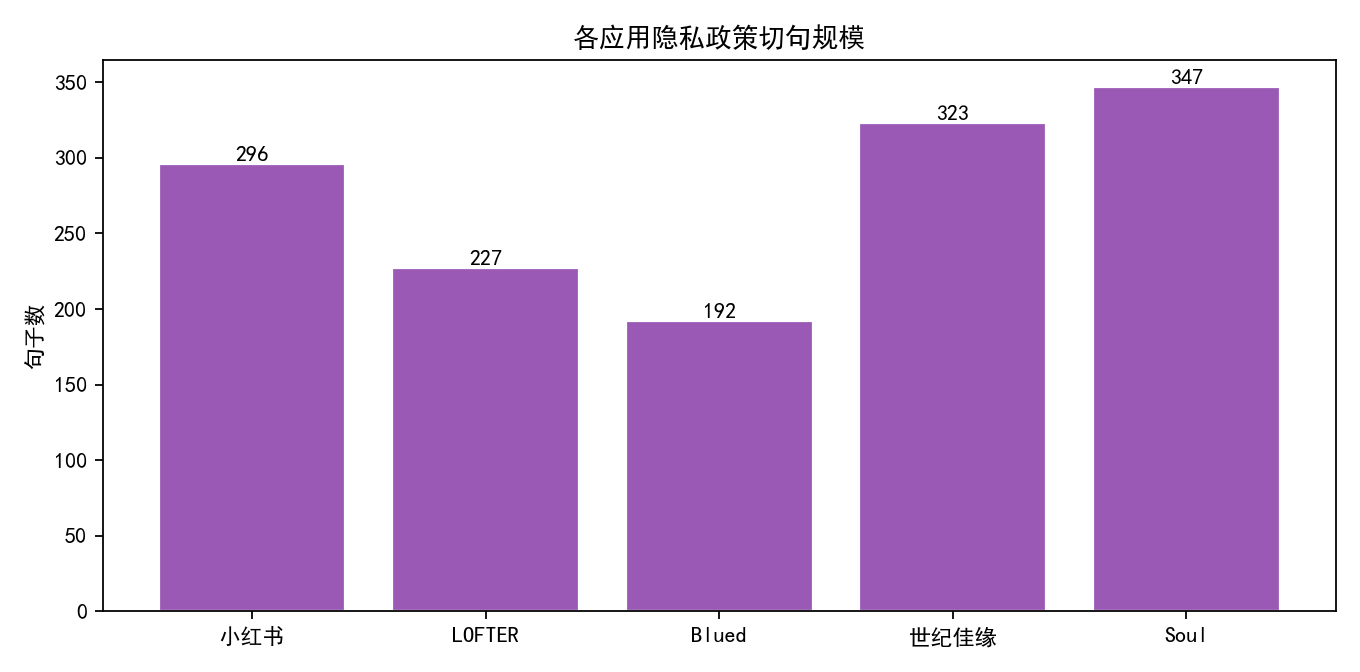
\includegraphics[width=0.42\linewidth]{fig_totals_by_app.png}
    \hfill
    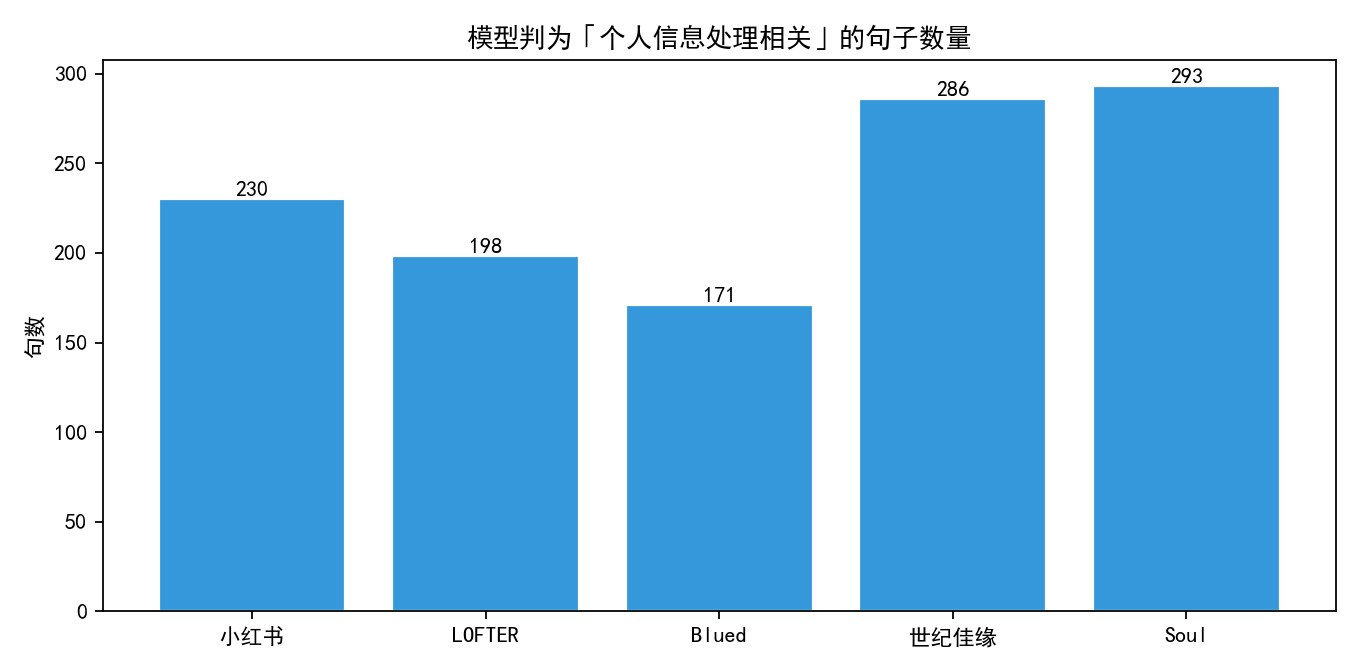
\includegraphics[width=0.42\linewidth]{fig_pii_true_by_app.png}
\end{frame}

\begin{frame}
    \frametitle{句级审计三标签汇总（大模型全量，共 1385 句）}
    \tiny
    \begin{tabularx}{\textwidth}{|l|r|r|r|r|r|}
        \toprule
        \textbf{应用} & \textbf{句数} & \textbf{incorrect 正例} & \textbf{incomplete 正例} & \textbf{inconsistent 正例} & \textbf{三标签合计} \\
        \midrule
        Blued 极速版 & 192 & 51 & 3 & 4 & 58 \\
        LOFTER       & 227 & 44 & 5 & 1 & 50 \\
        Soul         & 347 & 87 & 11 & 6 & 104 \\
        世纪佳缘     & 323 & 53 & 2 & 0 & 55 \\
        小红书       & 296 & 109 & 9 & 2 & 120 \\
        \midrule
        \textbf{合计} & \textbf{1385} & \textbf{344} & \textbf{30} & \textbf{13} & \textbf{387} \\
        \bottomrule
    \end{tabularx}
    \vspace{0.35em}
    \scriptsize
    \begin{itemize}
        \item 占全库比例（近似）：\textbf{incorrect 24.8\%}，\textbf{incomplete 2.2\%}，\textbf{inconsistent 0.9\%}（三标签可同句为 1，故分行加总可大于句数）。
        \item \textbf{小红书} incorrect 计数相对突出；\textbf{世纪佳缘} 无 inconsistent 正例。
    \end{itemize}
\end{frame}

\begin{frame}
    \frametitle{可视化：规则 vs 模型占比（历史汇总图）}
    \begin{columns}
        \begin{column}{0.52\textwidth}
            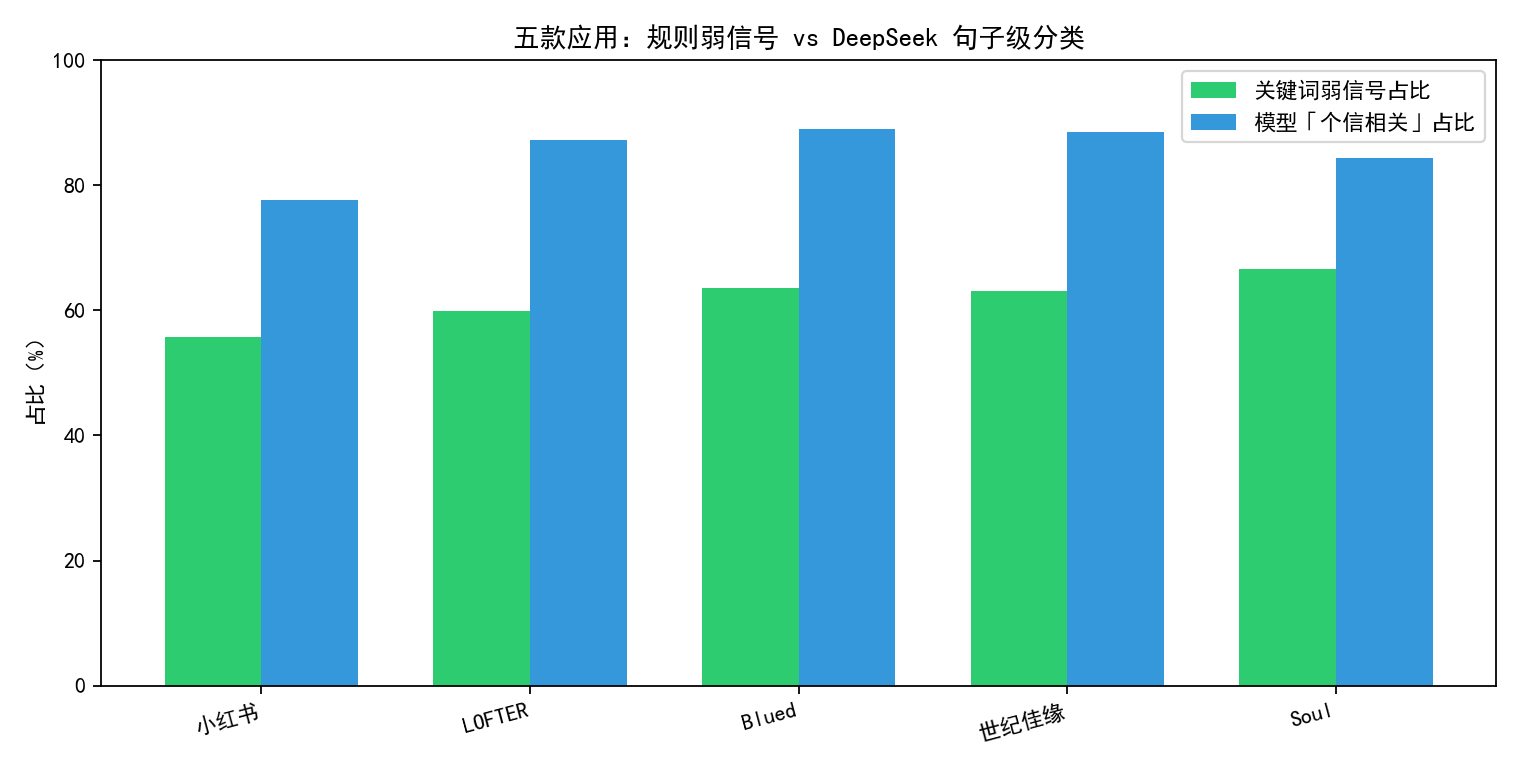
\includegraphics[width=\linewidth]{fig_ratios_by_app.png}
        \end{column}
        \begin{column}{0.46\textwidth}
            \scriptsize
            \begin{itemize}
                \item 绿柱：\textbf{规则弱信号}命中占比；蓝柱：\textbf{模型判定为个信相关}占比。
                \item 用于观察\textbf{弱规则与 LLM} 的差异，辅助送标优先级解释。
            \end{itemize}
        \end{column}
    \end{columns}
\end{frame}

\begin{frame}
    \frametitle{可视化：以 Soul 为例——分类与句长}
    \begin{columns}
        \begin{column}{0.5\textwidth}
            \centering
            
\includegraphics[width=\linewidth]{soul_detail/stats_counts.png}
        \end{column}
        \begin{column}{0.5\textwidth}
            \centering
            
\includegraphics[width=\linewidth]{soul_detail/sentence_length_hist.png}
        \end{column}
    \end{columns}
\end{frame}

\begin{frame}
	\frametitle{分析标准：核心内容要求（1-8）}
	\tiny
	\begin{tabularx}{\textwidth}{|c|X|c|X|}
		\toprule
		\textbf{序号} & \textbf{内容要求} & \textbf{对应法条} & \textbf{规范要点} \\
		\midrule
		\multicolumn{4}{|c|}{\textbf{一、隐私政策的核心内容要求（必须告知的事项）}} \\
		\midrule
		1 & 个人信息处理者的身份与联系方式 & 第十七条第一款第一项 & 明确运营主体，并提供有效联系方式 \\
		\midrule
		2 & 个人信息的处理目的、方式、种类与保存期限 & 第十七条第一款第二项 & 目的具体明确、方式清晰、种类逐项列出、保存期限最短必要 \\
		\midrule
		3 & 用户行使权利的方式和程序 & 第十七条第一款第三项 & 明确告知如何行使各项权利，提供便捷申请渠道 \\
		\midrule
		4 & 法律、行政法规规定的其他事项 & 第十七条第一款第四项 & 关注配套法规（《网络安全法》《数据安全法》等） \\
		\midrule
		5 & 查阅复制权行使方式 & 第四十五条 & 告知如何查阅、复制个人信息，提供便捷申请渠道 \\
		\midrule
		6 & 更正补充权行使方式 & 第四十六条 & 告知如何申请更正或补充不准确、不完整的个人信息 \\
		\midrule
		7 & 删除权行使方式 & 第四十七条 & 告知删除情形及具体申请路径、处理时限 \\
		\midrule
		8 & 撤回同意权行使方式 & 第十五条 & 撤回渠道应与同意方式同等便捷，不影响其他功能 \\
		\bottomrule
	\end{tabularx}
\end{frame}

\begin{frame}
	\frametitle{分析标准：特定情形额外告知（9-16）}
	\tiny
	\begin{tabularx}{\textwidth}{|c|X|c|X|}
		\toprule
		\textbf{序号} & \textbf{内容要求} & \textbf{对应法条} & \textbf{规范要点} \\
		\midrule
		\multicolumn{4}{|c|}{\textbf{二、针对特定情形或信息的额外告知要求}} \\
		\midrule
		9 & 处理敏感个人信息 & 第三十条 & 告知处理必要性及对个人权益的影响 \\
		\midrule
		10 & 向境外提供个人信息 & 第三十九条 & 告知境外接收方信息，并取得单独同意 \\
		\midrule
		11 & 不满14周岁未成年人信息 & 第三十一条 & 制定专门规则，取得监护人同意 \\
		\midrule
		12 & 委托处理、共同处理、因合并/分立转移信息 & 第二十一、二十二、二十三条 & 告知接收方信息，包括名称、联系方式、处理目的等 \\
		\midrule
		13 & 自动化决策（如个性化推荐） & 第二十四条 & 保证透明度与公平公正，提供非个性化选项 \\
		\midrule
		14 & 公开披露个人信息 & 第二十五条 & 原则上应取得单独同意，告知目的、种类及影响 \\
		\midrule
		15 & 已公开信息处理规则 & 第二十七条 & 遵循合理性原则，不得超出合理范围 \\
		\midrule
		16 & 数据泄露应急措施 & 第五十七条（建议） & 明确泄露通知流程，包括通知方式、时限及补救措施 \\
		\bottomrule
	\end{tabularx}
\end{frame}

\begin{frame}
	\frametitle{分析标准：格式与表述规范（17-22）}
	\tiny
	\begin{tabularx}{\textwidth}{|c|X|c|X|}
		\toprule
		\textbf{序号} & \textbf{内容要求} & \textbf{对应法条} & \textbf{规范要点} \\
		\midrule
		\multicolumn{4}{|c|}{\textbf{三、隐私政策的格式与表述规范}} \\
		\midrule
		17 & 显著清晰，易于理解 & 第十七条 & 语言平实易懂，展示方式显著，结构清晰 \\
		\midrule
		18 & 真实、准确、完整 & 第十七条 & 内容与实际处理实践完全一致 \\
		\midrule
		19 & 公开且便于查阅保存 & 第十七条第三款 & 长期公开在易于访问位置，提供离线保存选项 \\
		\midrule
		20 & 获得同意的规范 & 第十四条、第二十九条 & 自愿明确作出同意，特定情形需单独同意 \\
		\midrule
		21 & 与产品功能界面联动 & 第七条 & 隐私政策条款与App内权限申请弹窗等保持一致 \\
		\midrule
		22 & 撤回同意便捷性 & 第十五条 & 撤回渠道与获取同意方式同等便捷 \\
		\bottomrule
	\end{tabularx}
\end{frame}

\begin{frame}
    \frametitle{可视化：Soul — 个信相关×规则（UMAP）与 22 项着色}
    \centering
    
\includegraphics[width=0.46\linewidth]{Soul/cluster_analysis/umap_hdbscan.png}
    \hfill
    
\includegraphics[width=0.46\linewidth]{Soul/cluster_analysis/umap_taxonomy_22.png}
    \vspace{0.25em}
    \scriptsize
    左：原 HDBSCAN 密度聚类图位置，改为同一 UMAP 上按\textbf{模型个信相关 × 规则弱信号}四象限着色（替代无监督簇）；右：按 22 项中\textbf{余弦相似度最大}的一项着色。
\end{frame}

\begin{frame}
    \frametitle{可视化：Blued 极速版 — UMAP 与密度聚类、22 项着色}
    \centering
    
\includegraphics[width=0.46\linewidth]{Blued极速版/cluster_analysis/umap_hdbscan.png}
    \hfill
    
\includegraphics[width=0.46\linewidth]{Blued极速版/cluster_analysis/umap_taxonomy_22.png}
    \vspace{0.25em}
    \scriptsize
    左：句向量 UMAP 后按 \textbf{HDBSCAN} 密度簇着色（噪声点为灰）；右：每句在 22 项中取\textbf{余弦相似度最大}的一项作为「主色」，用于观察语义是否与合规维度对齐。
\end{frame}

\begin{frame}
    \frametitle{可视化：LOFTER — UMAP 与密度聚类、22 项着色}
    \centering
    
\includegraphics[width=0.46\linewidth]{LOFTER/cluster_analysis/umap_hdbscan.png}
    \hfill
    
\includegraphics[width=0.46\linewidth]{LOFTER/cluster_analysis/umap_taxonomy_22.png}
    \vspace{0.25em}
    \scriptsize
    左：句向量 UMAP 后按 \textbf{HDBSCAN} 密度簇着色（噪声点为灰）；右：每句在 22 项中取\textbf{余弦相似度最大}的一项作为「主色」，用于观察语义是否与合规维度对齐。
\end{frame}

\begin{frame}
    \frametitle{可视化：世纪佳缘 — UMAP 与密度聚类、22 项着色}
    \centering
    
\includegraphics[width=0.46\linewidth]{世纪佳缘/cluster_analysis/umap_hdbscan.png}
    \hfill
    
\includegraphics[width=0.46\linewidth]{世纪佳缘/cluster_analysis/umap_taxonomy_22.png}
    \vspace{0.25em}
    \scriptsize
    左：句向量 UMAP 后按 \textbf{HDBSCAN} 密度簇着色（噪声点为灰）；右：每句在 22 项中取\textbf{余弦相似度最大}的一项作为「主色」，用于观察语义是否与合规维度对齐。
\end{frame}

\begin{frame}
    \frametitle{可视化：小红书 — UMAP 与密度聚类、22 项着色}
    \centering
    
\includegraphics[width=0.46\linewidth]{小红书/cluster_analysis/umap_hdbscan.png}
    \hfill
    
\includegraphics[width=0.46\linewidth]{小红书/cluster_analysis/umap_taxonomy_22.png}
    \vspace{0.25em}
    \scriptsize
    左：句向量 UMAP 后按 \textbf{HDBSCAN} 密度簇着色（噪声点为灰）；右：每句在 22 项中取\textbf{余弦相似度最大}的一项作为「主色」，用于观察语义是否与合规维度对齐。
\end{frame}

\begin{frame}
    \frametitle{22 项合组 UMAP：多种聚合方案}
    \scriptsize
    \begin{itemize}
        \item \textbf{内容交叉合组}（各应用页\textbf{上排左图}）：\textbf{核心告知与行权路径} \{2,3,5,6,7,8\}；\textbf{特定告知与单独同意} \{9,10,14,20\}；\textbf{决策透明与用户控制} \{13,8,22\}。同一合组内各分点\textbf{同色}；灰色为最近邻项不在上述并集内（如项 1、4、11--12、15--19、21 等）。
        \item \textbf{格式 / 核心 / 增强}（各应用页\textbf{上排右图}）：\textbf{格式与可执行性基础} \{17,18,19,21,22\}；\textbf{核心告知义务} \{1--8\}；\textbf{增强告知与特殊程序义务} \{9--16,20\}。三组\textbf{互斥覆盖} 1--22（与上一种交叉视角不同）。
        \item \textbf{重叠项处理}：仅「内容交叉」方案中 8、22 等跨定义时按\textbf{先列出的合组优先}；「格式/核心/增强」与\textbf{六分（数据驱动）}各自内部无歧义重叠。
        \item \textbf{实现要点}：句向量 $\rightarrow$ UMAP 二维坐标；每句对 22 项的相似度来自\textbf{句向量与法参考段向量的余弦相似度}；合组图在统一配色规则下\textbf{按应用批量出图}便于对照。
    \end{itemize}
\end{frame}


\begin{frame}
    \frametitle{六分命名大类：22 项归属表}
    \tiny
    \begin{tabularx}{\textwidth}{|X|X|}
        \toprule
        \textbf{命名大类} & \textbf{所含标准序号（简要主题）} \\
        \midrule
        信息处理基础与台账 & \textbf{2, 5, 18, 19} — 处理目的/方式/种类/期限与查阅复制；真实准确完整；公开便于查阅保存 \\
        \midrule
        用户控制与算法交互核心 & \textbf{7, 8, 13, 21} — 删除权、撤回同意；自动化决策；与产品界面联动 \\
        \midrule
        未成年人保护专项 & \textbf{11} — 不满 14 周岁未成年人信息 \\
        \midrule
        高风险场景及单独同意 & \textbf{9, 14, 15, 20} — 敏感个人信息；公开披露；已公开信息处理；取得同意的规范 \\
        \midrule
        主体告知与复合程序要求 & \textbf{1, 3, 4, 6, 10, 12, 16, 17} — 身份联系方式、行权程序、其他法定事项、更正补充、出境、委托/共同/转移、泄露应急、显著清晰 \\
        \midrule
        撤回同意便捷性专项 & \textbf{22} — 撤回与取得同意同等便捷 \\
        \bottomrule
    \end{tabularx}
    
\end{frame}

\begin{frame}[shrink=5]
    \frametitle{合组 UMAP：Blued 极速版}
    \vspace{-0.35em}
    \begin{columns}[T]
        \begin{column}{0.5\textwidth}
            \centering
            
\includegraphics[width=0.96\linewidth]{Blued极速版/cluster_analysis/umap_taxonomy_merge_cross.png}
        \end{column}
        \begin{column}{0.5\textwidth}
            \centering
            
\includegraphics[width=0.96\linewidth]{Blued极速版/cluster_analysis/umap_taxonomy_merge_layers.png}
        \end{column}
    \end{columns}
    \vspace{-0.1em}
    \centering
    
\includegraphics[width=0.82\linewidth]{Blued极速版/cluster_analysis/umap_taxonomy_merge_data_driven.png}
\end{frame}

\begin{frame}[shrink=5]
    \frametitle{合组 UMAP：LOFTER}
    \vspace{-0.35em}
    \begin{columns}[T]
        \begin{column}{0.5\textwidth}
            \centering
            
\includegraphics[width=0.96\linewidth]{LOFTER/cluster_analysis/umap_taxonomy_merge_cross.png}
        \end{column}
        \begin{column}{0.5\textwidth}
            \centering
            
\includegraphics[width=0.96\linewidth]{LOFTER/cluster_analysis/umap_taxonomy_merge_layers.png}
        \end{column}
    \end{columns}
    \vspace{-0.1em}
    \centering
    
\includegraphics[width=0.82\linewidth]{LOFTER/cluster_analysis/umap_taxonomy_merge_data_driven.png}
\end{frame}

\begin{frame}[shrink=5]
    \frametitle{合组 UMAP：Soul}
    \vspace{-0.35em}
    \begin{columns}[T]
        \begin{column}{0.5\textwidth}
            \centering
            
\includegraphics[width=0.96\linewidth]{Soul/cluster_analysis/umap_taxonomy_merge_cross.png}
        \end{column}
        \begin{column}{0.5\textwidth}
            \centering
            
\includegraphics[width=0.96\linewidth]{Soul/cluster_analysis/umap_taxonomy_merge_layers.png}
        \end{column}
    \end{columns}
    \vspace{-0.1em}
    \centering
    
\includegraphics[width=0.82\linewidth]{Soul/cluster_analysis/umap_taxonomy_merge_data_driven.png}
\end{frame}

\begin{frame}[shrink=5]
    \frametitle{合组 UMAP：世纪佳缘}
    \vspace{-0.35em}
    \begin{columns}[T]
        \begin{column}{0.5\textwidth}
            \centering
            
\includegraphics[width=0.96\linewidth]{世纪佳缘/cluster_analysis/umap_taxonomy_merge_cross.png}
        \end{column}
        \begin{column}{0.5\textwidth}
            \centering
            
\includegraphics[width=0.96\linewidth]{世纪佳缘/cluster_analysis/umap_taxonomy_merge_layers.png}
        \end{column}
    \end{columns}
    \vspace{-0.1em}
    \centering
    
\includegraphics[width=0.82\linewidth]{世纪佳缘/cluster_analysis/umap_taxonomy_merge_data_driven.png}
\end{frame}

\begin{frame}[shrink=5]
    \frametitle{合组 UMAP：小红书}
    \vspace{-0.35em}
    \begin{columns}[T]
        \begin{column}{0.5\textwidth}
            \centering
            
\includegraphics[width=0.96\linewidth]{小红书/cluster_analysis/umap_taxonomy_merge_cross.png}
        \end{column}
        \begin{column}{0.5\textwidth}
            \centering
            
\includegraphics[width=0.96\linewidth]{小红书/cluster_analysis/umap_taxonomy_merge_layers.png}
        \end{column}
    \end{columns}
    \vspace{-0.1em}
    \centering
    
\includegraphics[width=0.82\linewidth]{小红书/cluster_analysis/umap_taxonomy_merge_data_driven.png}
\end{frame}



\begin{frame}
    \frametitle{可视化：Soul — 审计优先级与三标签正例图}
    \begin{columns}
        \begin{column}{0.5\textwidth}
            \centering
            
\includegraphics[width=\linewidth]{Soul/cluster_analysis/umap_audit_priority.png}
        \end{column}
        \begin{column}{0.5\textwidth}
            \centering
            
\includegraphics[width=\linewidth]{Soul/figures/audit_positive_counts.png}
        \end{column}
    \end{columns}
    \vspace{0.2em}
    \scriptsize
    左：按审计优先级着色（无三标签 / incorrect / incomplete / inconsistent）；右：\textbf{该应用全量审计结果}上各 Data Safety 标签取\textbf{正例}的句数柱状图（非送标抽样）。
\end{frame}

\begin{frame}
    \frametitle{可视化：全量句级审计（一）— 各应用三标签正例计数}
    \centering
    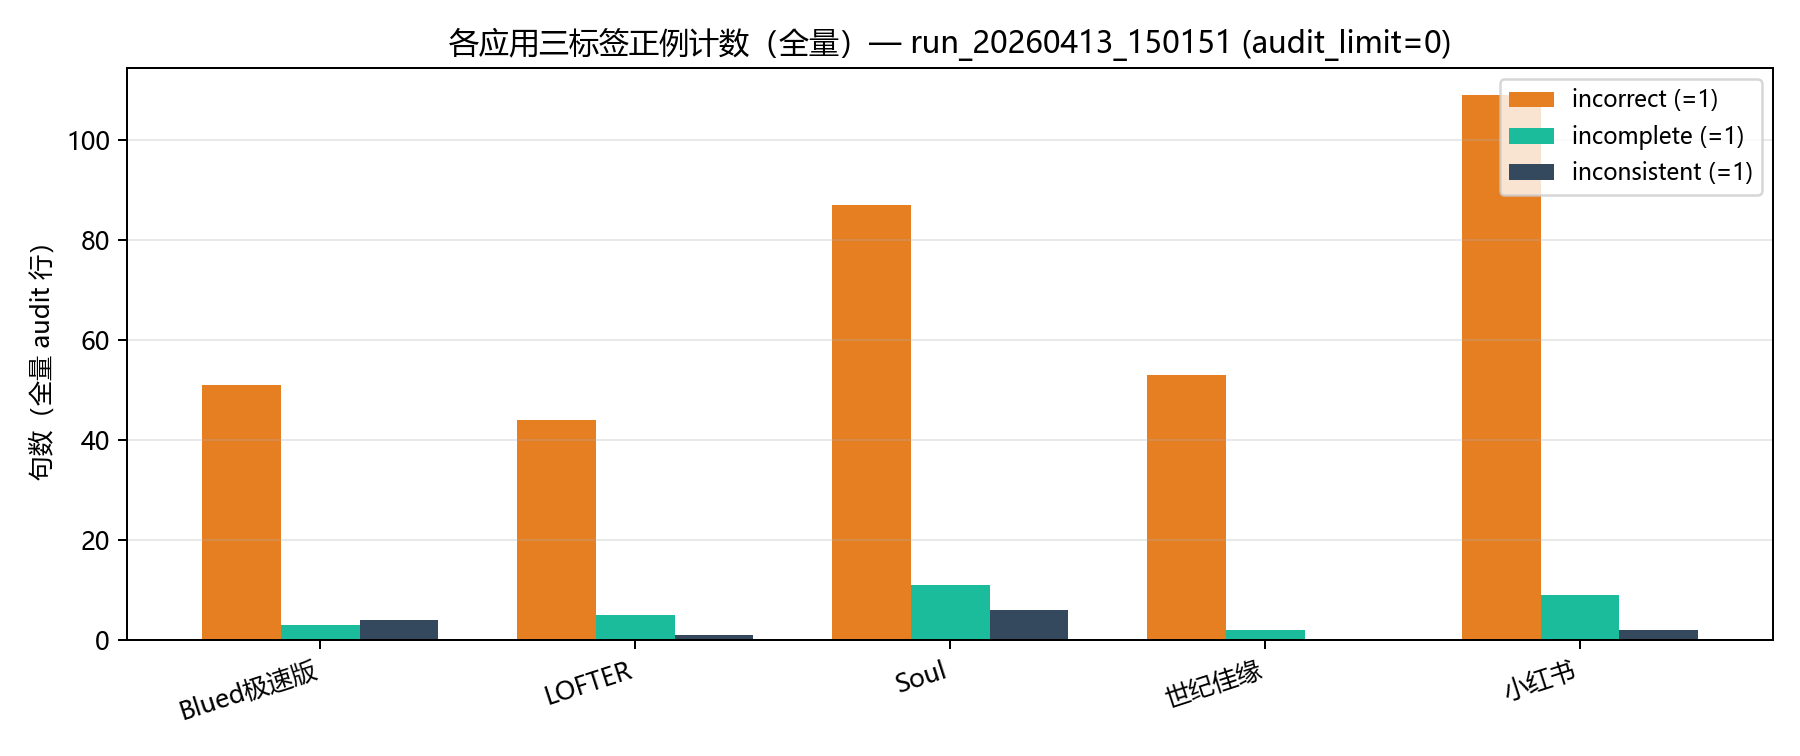
\includegraphics[width=0.95\linewidth]{fig_audit_full_grouped_by_app.png}
    \vspace{0.25em}
    \scriptsize
    由五应用\textbf{全量句级审计表}汇总得到各应用三标签正例计数（分组柱状图）。
\end{frame}

\begin{frame}
    \frametitle{可视化：全量句级审计（二）— 正例率与全库合计}
    \begin{columns}
        \begin{column}{0.56\textwidth}
            \centering
            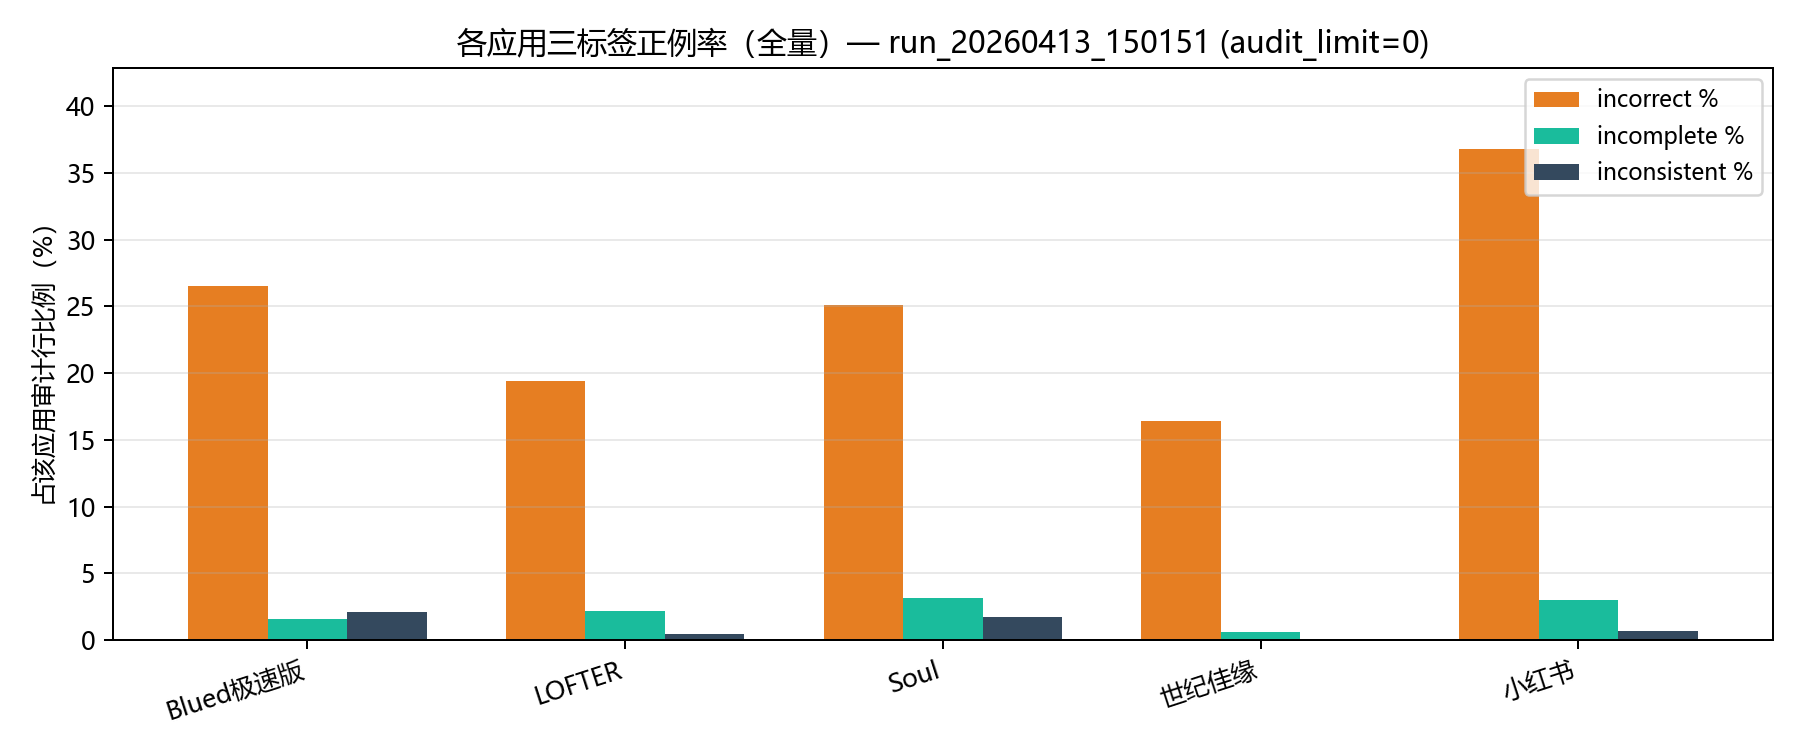
\includegraphics[width=\linewidth]{fig_audit_full_rates_by_app.png}
        \end{column}
        \begin{column}{0.42\textwidth}
            \centering
            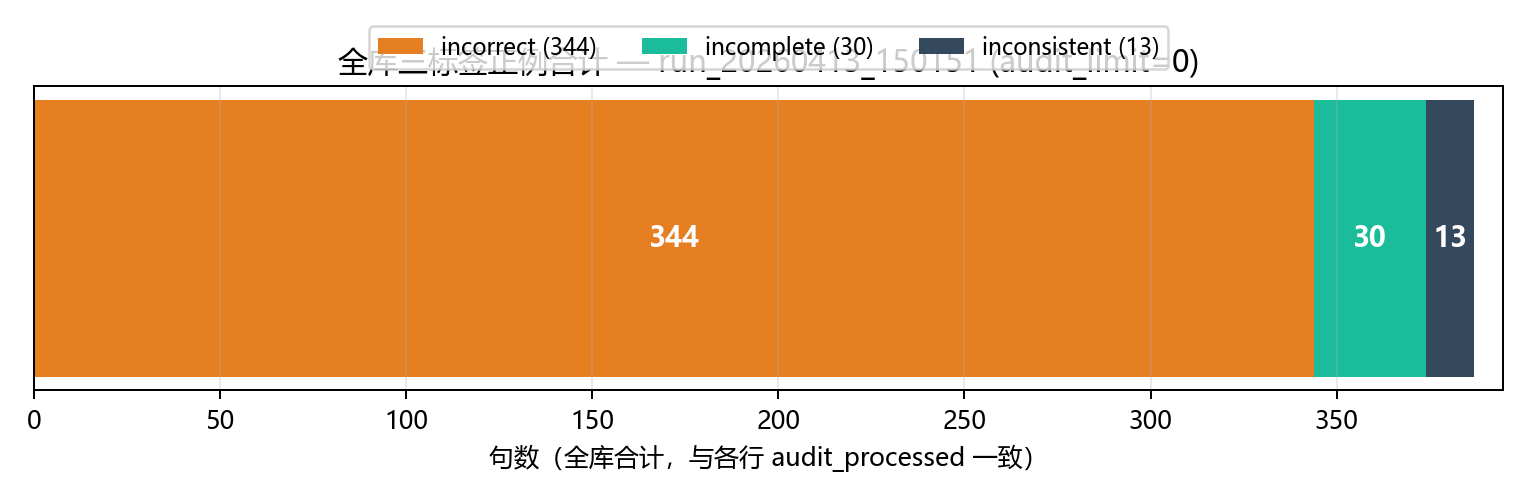
\includegraphics[width=\linewidth]{fig_audit_full_totals_stacked.png}
        \end{column}
    \end{columns}
    \vspace{0.2em}
    \scriptsize
    左：各标签正例占该应用\textbf{全量审计句}的比例；右：五应用合并后三标签正例句数（\textbf{344 + 30 + 13}，与结果表一致）。
\end{frame}

\begin{frame}
    \begin{center}
        {\Huge 感谢聆听！}
    \end{center}
\end{frame}

\end{document}
